%===============================================================================
% LaTeX sjabloon voor de bachelorproef toegepaste informatica aan HOGENT
% Meer info op https://github.com/HoGentTIN/latex-hogent-report
%===============================================================================

\documentclass[dutch,dit,thesis]{hogentreport}

% TODO:
% - If necessary, replace the option `dit`' with your own department!
%   Valid entries are dbo, dbt, dgz, dit, dlo, dog, dsa, soa
% - If you write your thesis in English (remark: only possible after getting
%   explicit approval!), remove the option "dutch," or replace with "english".

\usepackage{lipsum} % For blind text, can be removed after adding actual content

%% Pictures to include in the text can be put in the graphics/ folder
\graphicspath{{../graphics/}}

%% For source code highlighting, requires pygments to be installed
%% Compile with the -shell-escape flag!
%% \usepackage[chapter]{minted}
%% If you compile with the make_thesis.{bat,sh} script, use the following
%% import instead:
\usepackage[chapter,outputdir=../output]{minted}
\usemintedstyle{solarized-light}

%% Formatting for minted environments.
\setminted{%
    autogobble,
    frame=lines,
    breaklines,
    linenos,
    tabsize=4
}

%% Ensure the list of listings is in the table of contents
\renewcommand\listoflistingscaption{%
    \IfLanguageName{dutch}{Lijst van codefragmenten}{List of listings}
}
\renewcommand\listingscaption{%
    \IfLanguageName{dutch}{Codefragment}{Listing}
}
\renewcommand*\listoflistings{%
    \cleardoublepage\phantomsection\addcontentsline{toc}{chapter}{\listoflistingscaption}%
    \listof{listing}{\listoflistingscaption}%
}

% Other packages not already included can be imported here

%%---------- Document metadata -------------------------------------------------
% TODO: Replace this with your own information
\author{Luka Deserranno}
\supervisor{Mevr. S. VanderMeersch}
\cosupervisor{Dhr. T. Aelbrecht}
\title[Een onderzoek naar cloudopslag]%
    {Alternatieven voor Dropbox bij Aquarius Zwemclub Lebbeke}
\academicyear{\advance\year by -1 \the\year--\advance\year by 1 \the\year}
\examperiod{1}
\degreesought{\IfLanguageName{dutch}{Professionele bachelor in de toegepaste informatica}{Bachelor of applied computer science}}
\partialthesis{false} %% To display 'in partial fulfilment'
%\institution{Internshipcompany BVBA.}

%% Add global exceptions to the hyphenation here
\hyphenation{back-slash}

%% The bibliography (style and settings are  found in hogentthesis.cls)
\addbibresource{bachproef.bib}            %% Bibliography file
\addbibresource{../voorstel/voorstel.bib} %% Bibliography research proposal
\defbibheading{bibempty}{}

%% Prevent empty pages for right-handed chapter starts in twoside mode
\renewcommand{\cleardoublepage}{\clearpage}

\renewcommand{\arraystretch}{1.2}

%% Content starts here.
\begin{document}

%---------- Front matter -------------------------------------------------------

\frontmatter

\hypersetup{pageanchor=false} %% Disable page numbering references
%% Render a Dutch outer title page if the main language is English
\IfLanguageName{english}{%
    %% If necessary, information can be changed here
    \degreesought{Professionele Bachelor toegepaste informatica}%
    \begin{otherlanguage}{dutch}%
       \maketitle%
    \end{otherlanguage}%
}{}

%% Generates title page content
\maketitle
\hypersetup{pageanchor=true}

%%=============================================================================
%% Voorwoord
%%=============================================================================

\chapter*{\IfLanguageName{dutch}{Woord vooraf}{Preface}}%
\label{ch:voorwoord}

Deze bachelorproef markeert het eindpunt van mijn opleiding Toegepaste Informatica en is tegelijk een weerspiegeling van mijn interesse in digitale efficiëntie binnen kleinschalige organisaties. Vanuit mijn persoonlijke betrokkenheid bij sportverenigingen merkte ik dat technologie vaak beperkt of omslachtig wordt ingezet. Toen ik hoorde over de uitdagingen bij Aquarius Zwemclub Lebbeke rond het delen van documenten, zag ik meteen een kans om met een praktische en duurzame oplossing aan de slag te gaan.

De keuze om een eigen toegangsbeheersysteem uit te werken in combinatie met een cloudopslagdienst was technisch uitdagend, maar bijzonder leerrijk. Vooral het opzetten van fijnmazige toegangsrechten en de integratie met een gebruiksvriendelijke backendstructuur hebben mijn inzicht in softwarearchitectuur sterk verdiept.

Ik wil graag enkele mensen bedanken die mij doorheen dit traject hebben ondersteund. In de eerste plaats mijn promotor Mevrouw S. VanderMeersch, voor haar constructieve begeleiding en waardevolle feedback. Ook veel dank aan Dhr. Thomas Aelbrecht, die niet alleen als co-promotor, maar ook als webmaster van AZL een onmisbare rol speelde in het aanleveren van context, technische vereisten en het testen van de oplossing in de praktijk.

Verder gaat mijn dank uit naar de lesgevers en medewerkers van AZL die meegewerkt hebben aan de evaluatie van het systeem. Tot slot wil ik ook mijn familie en vrienden bedanken voor hun aanmoediging en geduld tijdens de vele uren achter mijn scherm.

Luka Deserranno \\
Academiejaar 2024–2025

%%=============================================================================
%% Samenvatting
%%=============================================================================

% TODO: De "abstract" of samenvatting is een kernachtige (~ 1 blz. voor een
% thesis) synthese van het document.
%
% Een goede abstract biedt een kernachtig antwoord op volgende vragen:
%
% 1. Waarover gaat de bachelorproef?
% 2. Waarom heb je er over geschreven?
% 3. Hoe heb je het onderzoek uitgevoerd?
% 4. Wat waren de resultaten? Wat blijkt uit je onderzoek?
% 5. Wat betekenen je resultaten? Wat is de relevantie voor het werkveld?
%
% Daarom bestaat een abstract uit volgende componenten:
%
% - inleiding + kaderen thema
% - probleemstelling
% - (centrale) onderzoeksvraag
% - onderzoeksdoelstelling
% - methodologie
% - resultaten (beperk tot de belangrijkste, relevant voor de onderzoeksvraag)
% - conclusies, aanbevelingen, beperkingen
%
% LET OP! Een samenvatting is GEEN voorwoord!

%%---------- Nederlandse samenvatting -----------------------------------------
%
% TODO: Als je je bachelorproef in het Engels schrijft, moet je eerst een
% Nederlandse samenvatting invoegen. Haal daarvoor onderstaande code uit
% commentaar.
% Wie zijn bachelorproef in het Nederlands schrijft, kan dit negeren, de inhoud
% wordt niet in het document ingevoegd.

\IfLanguageName{english}{%
\selectlanguage{dutch}
\chapter*{Samenvatting}
\lipsum[1-4]
\selectlanguage{english}
}{}

%%---------- Samenvatting -----------------------------------------------------
% De samenvatting in de hoofdtaal van het document

\chapter*{\IfLanguageName{dutch}{Samenvatting}{Abstract}}

Aquarius Zwemclub Lebbeke (AZL) maakt momenteel gebruik van Dropbox voor het delen van bestanden tussen lesgevers. Deze oplossing kent echter meerdere beperkingen, 
waaronder verouderde toegangsrechten, gebrekkige integratie met bestaande systemen en een lage gebruiksvriendelijkheid voor lesgevers zonder Dropbox-account. 
Om deze problemen aan te pakken, werd in deze bachelorproef gezocht naar een alternatieve cloudopslagoplossing die beter inspeelt op de noden van AZL.

De centrale onderzoeksvraag luidt: \textbf{Hoe kan AZL een cloudopslagoplossing implemente- ren die zorgt voor een beter beheer van de toe- gang tot bestanden, eenvoudig integreert met de bestaande systemen, en gebruiksvriendelijk is voor alle lesgevers, zonder dat zij hiervoor een extra account hoeven aan te maken?}

Om tot een antwoord te komen werd een gestructureerde methode toegepast. Eerst werd via een literatuurstudie een longlist van mogelijke oplossingen samengesteld. 
Vervolgens werden de functionele en niet-functionele vereisten van AZL in kaart gebracht, waarop een shortlist van de meest geschikte alternatieven werd opgesteld. 
Hieruit werd Nextcloud geselecteerd als meest veelbelovende optie. Ter evaluatie werd een proof of concept (PoC) ontwikkeld en getest binnen de 
bestaande IT-infrastructuur van AZL.

De resultaten tonen aan dat Nextcloud door zijn open-source karakter, flexibiliteit en uitgebreide mogelijkheden voor toegangsbeheer een sterke match vormt voor AZL. 
De oplossing zorgde voor een vereenvoudigd beheer van toegangsrechten, verbeterde integratie met de bestaande webapplicatie en een gebruiksvriendelijke ervaring voor 
de lesgevers, zonder dat zij een extra account hoefden aan te maken.

Op basis van dit onderzoek kan geconcludeerd worden dat Nextcloud een geschikte en toekomstbestendige oplossing is voor AZL. De implementatie ervan biedt niet 
alleen technische voordelen, maar draagt ook bij aan een efficiëntere werking en vermindert de administratieve last. Voor andere verenigingen met vergelijkbare 
noden kan dit onderzoek dienen als leidraad bij de keuze voor een geschikte cloudopslagoplossing.

%---------- Inhoud, lijst figuren, ... -----------------------------------------

\tableofcontents

% In a list of figures, the complete caption will be included. To prevent this,
% ALWAYS add a short description in the caption!
%
%  \caption[short description]{elaborate description}
%
% If you do, only the short description will be used in the list of figures

\listoffigures

% If you included tables and/or source code listings, uncomment the appropriate
% lines.
\listoftables

\listoflistings

% Als je een lijst van afkortingen of termen wil toevoegen, dan hoort die
% hier thuis. Gebruik bijvoorbeeld de ``glossaries'' package.
% https://www.overleaf.com/learn/latex/Glossaries

%---------- Kern ---------------------------------------------------------------

\mainmatter{}

% De eerste hoofdstukken van een bachelorproef zijn meestal een inleiding op
% het onderwerp, literatuurstudie en verantwoording methodologie.
% Aarzel niet om een meer beschrijvende titel aan deze hoofdstukken te geven of
% om bijvoorbeeld de inleiding en/of stand van zaken over meerdere hoofdstukken
% te verspreiden!

%%=============================================================================
%% Inleiding
%%=============================================================================

\chapter{\IfLanguageName{dutch}{Inleiding}{Introduction}}%
\label{ch:inleiding}

Binnen sportverenigingen speelt een efficiënte digitale werking een steeds belangrijkere rol. Documenten zoals lesplanningen, presentaties en evaluaties dienen vlot gedeeld en beheerd te worden om de dagelijkse werking te ondersteunen. Bij Aquarius Zwemclub Lebbeke (AZL) wordt hiervoor momenteel gebruikgemaakt van Dropbox. Hoewel dit platform aanvankelijk voldeed aan de basisbehoeften, ondervindt AZL vandaag structurele problemen zoals verouderde toegangsrechten, het ontbreken van integratie met bestaande systemen, en beperkte toegankelijkheid voor lesgevers zonder Dropbox-account. Deze uitdagingen zorgen voor een verhoogde administratieve werklast en verhinderen een efficiënte samenwerking.

AZL beschikt over een bestaande IT-infrastructuur die onder andere bestaat uit een WordPress-website, een op maat ontwikkelde webapplicatie en hosting via DigitalOcean. De afwezigheid van een geïntegreerde en centraal beheerde cloudopslagoplossing leidt tot extra manueel werk bij het beheren van gebruikers en hun toegangsrechten. Bovendien missen lesgevers vaak de juiste middelen om zonder drempels toegang te krijgen tot de noodzakelijke documenten. 

Het doel van deze bachelorproef is om een duurzame, veilige en gebruiksvriendelijke cloudopslagoplossing te selecteren die niet alleen aansluit bij de specifieke noden van AZL, maar ook eenvoudig te integreren is met de bestaande infrastructuur. Hierbij wordt bijzondere aandacht besteed aan kostenbeheersing, schaalbaarheid en onderhoudsvriendelijkheid. Uiteindelijk wordt de gekozen oplossing geïmplementeerd in een proof of concept (PoC), waarmee getest wordt of deze effectief bijdraagt aan een vlottere werking van AZL.

\section{Probleemstelling}%
\label{sec:probleemstelling}

Aquarius Zwemclub Lebbeke is een lokale sportvereniging die afhankelijk is van digitale bestanden voor het ondersteunen van haar lessen en trainingen. Het huidige gebruik van Dropbox biedt niet langer een toekomstgerichte oplossing. Toegangsrechten worden niet automatisch bijgewerkt, integratie met bestaande toepassingen ontbreekt, en niet elke lesgever beschikt over een Dropbox-account. Dit alles leidt tot een verhoogde werkdruk voor de beheerders en zorgt ervoor dat niet alle lesgevers even eenvoudig toegang hebben tot de benodigde documenten.

Deze bachelorproef richt zich daarom exclusief op AZL en heeft als doel een cloudopslagoplossing te onderzoeken die eenvoudig te beheren is, goed integreert met de huidige infrastructuur en gebruiksvriendelijk is voor alle betrokkenen. De doelgroep bestaat uit de lesgevers en beheerders van AZL, met als belangrijkste belanghebbende de webmaster van de club die instaat voor het technisch beheer van de systemen.

\section{Onderzoeksvraag}%
\label{sec:onderzoeksvraag}

De centrale onderzoeksvraag van deze bachelorproef luidt:

\begin{quote}
Welke cloudopslagoplossing biedt Aquarius Zwemclub Lebbeke de beste balans tussen gebruiksvriendelijkheid, kostenbeheersing, integratie met bestaande systemen en efficiënt gebruikersbeheer?
\end{quote}

Om deze hoofdvraag te beantwoorden, worden volgende deelvragen onderzocht:

\begin{itemize}
  \item Welke cloudopslagoplossingen zijn geschikt voor een kleine sportvereniging zoals AZL?
  \item Wat zijn de voor- en nadelen van de verschillende beschikbare oplossingen?
  \item Hoe kan een cloudopslagoplossing geïntegreerd worden met de bestaande systemen van AZL?
  \item Hoe kan het toegangsbeheer efficiënt, veilig en up-to-date worden gehouden?
  \item Wat zijn de kosten van de verschillende oplossingen en hoe verhouden deze zich tot het beschikbare budget van AZL?
\end{itemize}

\section{Onderzoeksdoelstelling}%
\label{sec:onderzoeksdoelstelling}

Deze bachelorproef heeft als doel het selecteren, implementeren en evalueren van een geschikte cloudopslagoplossing voor AZL. Het einddoel is om een proof of concept (PoC) te ontwikkelen waarin de gekozen oplossing geïntegreerd wordt in de bestaande IT-omgeving van AZL. Het succes van het onderzoek wordt bepaald aan de hand van de volgende criteria:

\begin{itemize}
  \item De oplossing biedt eenvoudig beheer van gebruikers en toegangsrechten.
  \item De oplossing integreert met de bestaande WordPress-website en webapplicatie van AZL.
  \item Lesgevers kunnen zonder bijkomende accounts vlot toegang krijgen tot de documenten.
  \item De oplossing blijft financieel haalbaar binnen het beperkte budget van AZL.
\end{itemize}

Het resultaat van deze bachelorproef bestaat uit een werkend prototype van de gekozen oplossing, een grondige evaluatie ervan binnen AZL en aanbevelingen voor een mogelijke volledige implementatie.

\section{\IfLanguageName{dutch}{Opzet van deze bachelorproef}{Structure of this bachelor thesis}}%
\label{sec:opzet-bachelorproef}

% Het is gebruikelijk aan het einde van de inleiding een overzicht te
% geven van de opbouw van de rest van de tekst. Deze sectie bevat al een aanzet
% die je kan aanvullen/aanpassen in functie van je eigen tekst.

De rest van deze bachelorproef is als volgt opgebouwd:

In Hoofdstuk~\ref{ch:stand-van-zaken} wordt een overzicht gegeven van de stand van zaken binnen het onderzoeksdomein, op basis van een literatuurstudie.

In Hoofdstuk~\ref{ch:methodologie} wordt de methodologie toegelicht en worden de gebruikte onderzoekstechnieken besproken om een antwoord te kunnen formuleren op de onderzoeksvragen.

% TODO: Vul hier aan voor je eigen hoofstukken, één of twee zinnen per hoofdstuk

In Hoofdstuk~\ref{ch:conclusie}, tenslotte, wordt de conclusie gegeven en een antwoord geformuleerd op de onderzoeksvragen. Daarbij wordt ook een aanzet gegeven voor toekomstig onderzoek binnen dit domein.
\chapter{\IfLanguageName{dutch}{Stand van zaken}{State of the art}}%
\label{ch:stand-van-zaken}

% Tip: Begin elk hoofdstuk met een paragraaf inleiding die beschrijft hoe
% dit hoofdstuk past binnen het geheel van de bachelorproef. Geef in het
% bijzonder aan wat de link is met het vorige en volgende hoofdstuk.

% Pas na deze inleidende paragraaf komt de eerste sectiehoofding.

Deze literatuurstudie onderzoekt beschikbare cloudopslagoplossingen die voldoen aan de specefieke behoeften van AZL. 
De focus ligt op integratiemogelijkheden met de bestaande Angular frontend en Node.js backend, gebruiksvriendelijkheid, efficiënt toegangsbeheer en kosteneffectiviteit. 
Deze studie vormt de basis voor het selecteren van een geschikte cloudopslagoplossing voor AZL.

\section{Huidige IT-infrastructuur bij AZL}
Aquarius Zwemclub Lebbeke (AZL) maakt momenteel gebruik van een eenvoudige maar doeltreffende IT-infrastructuur:
\begin{itemize}
    \item \textbf{Hosting}: De webapplicatie gebouwd met Angular en Node.js zijn gehost op DigitalOcean.
    \item \textbf{E-mailservices}: De SMTP-server wordt gehost bij AWS, dit omdat deze functionaliteit niet beschikbaar is bij DigitalOcean.
    \item \textbf{Cloudopslag}: Voor het delen van bestanden tussen lesgevers wordt Dropbox gebruikt.
    \item \textbf{Authenticatie en autorisatie}: De webapplicatie maakt gebruik van een zelfgebouwd authenticatiesysteem, er wordt dus geen gebruik gemaakt van externe diensten. Binnen de applicatie wordt reeds gebruik gemaakt van rollen.
\end{itemize}
Hoewel deze infrastructuur functioneel is, kent AZL verschillende uitdagingen: er is geen integratie tussen de cloudopslag en de 
webapplicatie, en geautomatiseerd toegangsbeheer ontbreekt. Een complete oplossing kan deze problemen aanpakken 
door integratie tussen de cloudopslag en de applicaties mogelijk te maken, wat zal zorgen voor een gebruiksvriendelijkere en efficiëntere werking.

\section{Integratie van cloudopslag in webapplicaties}
\subsection{Architecturele overwegingen}
Bij het integreren van cloudopslag in webapplicaties is de architectuur een cruciale factor. Integratie kan worden gerealiseerd via drie primaire architecturele benaderingen:
\begin{itemize}
  \item \textbf{API-gebaseerde integratie}: De webapplicatie communiceert via API's met de cloudopslag.
  \item \textbf{SDK-gebaseerde integratie}: Software Development Kits (SDK's) vereenvoudigen de communicatie tussen applicatie en cloudopslag.
  \item \textbf{Hybride integratie}: Combinatie van API's en SDK's voor optimale flexibiliteit.
\end{itemize}

\subsection{Frontend frameworks voor bestandsbeheer}
Voor de interactie en visualisatie van de cloudopslag in Angular zijn verschillende UI-frameworks beschikbaar. Dit maakt het ontwikkelen minder complex daar er al een component voor bestaat.

\subsubsection{ngx-explorer}
\texttt{ngx-explorer} is een Angular-component die uitgebreide ondersteuning biedt voor het beheren en visualiseren van bestanden in een cloudomgeving. De implementatie verloopt in enkele eenvoudige stappen:
  
\textbf{Configuratie en gebruik}: Plaats de component in je template met de tag \texttt{<ngx-explorer>}. Via inputparameters en events kun je onder andere:
  \begin{itemize}
    \item De startmap en toegangsrechten instellen.
    \item Thema’s en stijlen aanpassen middels CSS-overschrijvingen.
    \item Evenementen zoals bestandsselectie of uploadstatus monitoren.
  \end{itemize}

Wat betreft aanpasbaarheid biedt \texttt{ngx-explorer} een solide basis:
\begin{itemize}
  \item De standaard UI heeft een gemiddelde flexibiliteit, maar door gebruik te maken van Angular's component-architectuur en uitgebreide CSS-opties is het relatief eenvoudig om de look en feel aan te passen.
  \item De uitgebreide documentatie en actieve onderhoudsondersteuning zorgen ervoor dat ontwikkelaars snel problemen kunnen oplossen en de component kunnen uitbreiden naar specifieke behoeften.
  \item De component ondersteunt integratie met diverse cloudopslagdiensten via zowel API's als SDK's, wat een hybride integratie mogelijk maakt en de schaalbaarheid van de applicatie waarborgt.
\end{itemize}

\section{Vergelijkende analyse van cloudopslagoplossingen}
Om een geschikte cloudopslagoplossing voor AZL te vinden, zijn verschillende cloudoplossingen beoordeeld op basis van criteria die specifiek aansluiten bij de uitdagingen en behoeften van de organisatie:
\begin{itemize}
    \item Geschikt zijn voor kleine tot middelgrote organisaties: De oplossing moet betaalbaar en beheersbaar zijn voor een sportvereniging met beperkte middelen.
    \item Naadloos geïntegreerd kunnen worden: De oplossing moet aansluiten op de bestaande WordPress-website en Angular-webapplicatie.
    \item Flexibel zijn in toegangsbeheer: De oplossing moet een efficiënte en veilige manier bieden om toegangsrechten te beheren, waarbij lesgevers eenvoudig kunnen worden toegevoegd of verwijderd.
    \item Gebruiksvriendelijk en technisch haalbaar zijn: De oplossing moet eenvoudig te gebruiken zijn voor lesgevers met beperkte technische kennis en flexibel genoeg voor de webmaster.
    \item Onderhoudsvriendelijk zijn: De oplossing moet eenvoudig te beheren zijn door de webmaster na de implementatie.
\end{itemize}
%%=============================================================================
%% Methodologie
%%=============================================================================

\chapter{\IfLanguageName{dutch}{Methodologie}{Methodology}}%
\label{ch:methodologie}

%% TODO: In dit hoofstuk geef je een korte toelichting over hoe je te werk bent
%% gegaan. Verdeel je onderzoek in grote fasen, en licht in elke fase toe wat
%% de doelstelling was, welke deliverables daar uit gekomen zijn, en welke
%% onderzoeksmethoden je daarbij toegepast hebt. Verantwoord waarom je
%% op deze manier te werk gegaan bent.
%% 
%% Voorbeelden van zulke fasen zijn: literatuurstudie, opstellen van een
%% requirements-analyse, opstellen long-list (bij vergelijkende studie),
%% selectie van geschikte tools (bij vergelijkende studie, "short-list"),
%% opzetten testopstelling/PoC, uitvoeren testen en verzamelen
%% van resultaten, analyse van resultaten, ...
%%
%% !!!!! LET OP !!!!!
%%
%% Het is uitdrukkelijk NIET de bedoeling dat je het grootste deel van de corpus
%% van je bachelorproef in dit hoofstuk verwerkt! Dit hoofdstuk is eerder een
%% kort overzicht van je plan van aanpak.
%%
%% Maak voor elke fase (behalve het literatuuronderzoek) een NIEUW HOOFDSTUK aan
%% en geef het een gepaste titel.

\lipsum[21-25]



% Voeg hier je eigen hoofdstukken toe die de ``corpus'' van je bachelorproef
% vormen. De structuur en titels hangen af van je eigen onderzoek. Je kan bv.
% elke fase in je onderzoek in een apart hoofdstuk bespreken.

%\input{...}
%\input{...}
%...

%%=============================================================================
%% Conclusie
%%=============================================================================

\chapter{Conclusie}
\label{ch:conclusie}

In deze bachelorproef wordt onderzocht welke cloudopslagoplossing Aquarius Zwemclub Lebbeke (AZL) de beste balans biedt tussen gebruiksvriendelijkheid, kostenbeheersing, integratie met bestaande systemen en efficiënt gebruikersbeheer. Vanuit de centrale onderzoeksvraag worden de vereisten van AZL in kaart gebracht en wordt een selectieproces doorlopen op basis van functionele en niet-functionele criteria. De MoSCoW-methode structureert en prioriteert deze criteria.

De bijdrage van dit onderzoek ligt in het opstellen van een praktijkgericht selectiekader voor cloudopslag in kleinschalige organisaties met beperkte middelen. Daarnaast wordt een proof of concept (PoC) ontwikkeld waarin DigitalOcean Spaces geïntegreerd is in een bestaande Angular/Node.js-omgeving, voorzien van een fijnmazig en uitbreidbaar toegangsbeheersysteem. Deze architectuur toont aan dat moderne cloudopslagfunctionaliteit — inclusief beveiliging en fijnmazige toegangscontrole — ook zonder dure licenties of complexe infrastructuur realiseerbaar is. Daarmee biedt dit werk concrete meerwaarde voor vrijwilligersverenigingen en sportclubs met gelijkaardige IT-behoeften.

De resultaten bevestigen grotendeels de initiële verwachtingen: het technisch integreren van een alternatieve opslagoplossing blijkt haalbaar en efficiënt. De integratie met de publieke WordPress-site valt buiten scope, maar vormt een logische volgende stap. In productie kunnen nog aandachtspunten opduiken rond gebruiksgemak, logging en foutafhandeling, waarvoor het systeem ruimte laat om verder geoptimaliseerd te worden.

Het onderzoek werpt ook nieuwe vragen op. Zo is het relevant om te verkennen hoe het systeem zich gedraagt bij schaalvergroting of piekbelasting. Een uitbreiding naar \textbf{federated sharing} — waarbij bestanden gedeeld worden over verschillende organisaties zonder dat ze op één centrale locatie worden opgeslagen — kan eveneens bijdragen tot bredere inzetbaarheid. Verder is het waardevol om te onderzoeken hoe het systeem eenvoudig overdraagbaar kan blijven binnen vrijwilligersorganisaties, waar regelmatig wissels in beheer plaatsvinden.

Samenvattend biedt deze bachelorproef een solide basis voor een toekomstgerichte cloudstrategie binnen AZL en soortgelijke verenigingen, met voldoende ruimte voor verdere validatie, uitbreiding en optimalisatie.


%---------- Bijlagen -----------------------------------------------------------

\appendix

\chapter{Onderzoeksvoorstel}

Het onderwerp van deze bachelorproef is gebaseerd op een onderzoeksvoorstel dat vooraf werd beoordeeld door de promotor. Dat voorstel is opgenomen in deze bijlage.

%% TODO: 
%\section*{Samenvatting}

% Kopieer en plak hier de samenvatting (abstract) van je onderzoeksvoorstel.

% Verwijzing naar het bestand met de inhoud van het onderzoeksvoorstel
%---------- Inleiding ---------------------------------------------------------

% TODO: Is dit voorstel gebaseerd op een paper van Research Methods die je
% vorig jaar hebt ingediend? Heb je daarbij eventueel samengewerkt met een
% andere student?
% Zo ja, haal dan de tekst hieronder uit commentaar en pas aan.

%\paragraph{Opmerking}

% Dit voorstel is gebaseerd op het onderzoeksvoorstel dat werd geschreven in het
% kader van het vak Research Methods dat ik (vorig/dit) academiejaar heb
% uitgewerkt (met medesturent VOORNAAM NAAM als mede-auteur).
% 

\section{Inleiding}%
\label{sec:inleiding}

Het efficiënt beheren van gegevens en bestanden wordt steeds belangrijker voor organisaties, 
inclusief kleinere organisaties zoals sportclubs. Aquarius Zwemclub Lebbeke (AZL) maakt momenteel 
gebruik van Dropbox om bestanden te delen tussen lesgevers, maar er zijn verschillende problemen. 
De toegangsrechten zijn niet altijd actueel, er is geen integratie met zowel de WordPress-website als de webapplicatie, en sommige 
lesgevers hebben geen Dropbox-account, waardoor ze geen toegang hebben tot de cloudomgeving. 
Dit leidt extra handmatig werk voor de beheerders.

Dit onderzoek richt zich op het vinden van een geschikt alternatief voor Dropbox dat beter aansluit 
bij de behoeften van AZL. Het doel is om een cloudopslagoplossing te vinden die eenvoudig te beheren is, 
die zorgt voor duidelijke en up-to-date toegangsrechten, en die goed integreert met de huidige systemen van de zwemclub. 
Dit zal het voor lesgevers makkelijker maken om toegang te krijgen tot de juiste bestanden en mappen, en tegelijkertijd de 
administratieve werklast voor de beheerders verlagen.

De centrale vraag in dit onderzoek is: \textit{Hoe kan AZL een cloudopslagoplossing implementeren die zorgt voor een beter beheer van de 
toegang tot bestanden, eenvoudig integreert met de bestaande systemen, en gebruiksvriendelijk is voor alle lesgevers, zonder dat zij hiervoor 
een extra account hoeven aan te maken?} Om deze vraag te beantwoorden, wordt onderzocht welke mogelijkheden er zijn om een cloudopslagoplossing 
te voorzien en hoe deze aansluiten bij de behoeften van AZL. Daarbij worden de voor- en nadelen van verschillende oplossingen geëvalueerd, 
evenals de integratiemogelijkheden met de bestaande systemen, het toegangsbeheer, en de kostprijs. Door deze aspecten in kaart te brengen, 
kan een weloverwogen keuze worden gemaakt voor een oplossing die de administratieve werklast vermindert en tegelijkertijd een optimale gebruikerservaring biedt.

Het doel van dit onderzoek is om verschillende cloudopslagoplossingen te vergelijken, de voor- en nadelen van elke oplossing te evalueren en uiteindelijk een werkend prototype (proof of concept) te ontwikkelen van de beste oplossing voor AZL. Het resultaat zal niet alleen een proof of concept bevatten, maar ook concrete aanbevelingen voor de implementatie van de gekozen oplossing.

%---------- Stand van zaken ---------------------------------------------------

\section{Literatuurstudie}%
\label{sec:literatuurstudie}

Binnen Aquarius Zwemclub Lebbeke (AZL) is er een dringende behoefte aan een cloudopslagoplossing die zowel gebruiksvriendelijk is als makkelijk kan worden geïntegreerd met hun bestaande webapplicatie. De oplossing moet de mogelijkheid bieden om documenten efficiënt te delen tussen lesgevers, terwijl ze ook voldoen aan de vereisten voor toegangsbeheer en beveiliging. Deze literatuurstudie onderzoekt vier populaire cloudopslagoplossingen: Dropbox, Amazon S3, Nextcloud en Microsoft OneDrive. We vergelijken deze op basis van integratiemogelijkheden met webapplicaties, kosten, toegangsbeheer, beveiliging en gebruiksvriendelijkheid.

\subsection{Dropbox}
Dropbox is een van de meest populaire cloudopslagoplossingen, bekend om zijn eenvoud en gebruiksvriendelijke interface. Het biedt een degelijke integratie met verschillende webapplicaties, zoals via Dropbox Business API's, die het mogelijk maken om bestanden eenvoudig te beheren en te delen binnen een webapplicatie. Er is echter een beperking op het gebied van diepgaande integratie en configuratie van geavanceerd toegangsbeheer.

Dropbox biedt beperkte ondersteuning voor gedetailleerd toegangsbeheer binnen webapplicaties, wat betekent dat het voor AZL lastig kan zijn om verschillende gebruikersrollen en gedetailleerde machtigingen in hun webapplicatie te beheren. Dropbox ondersteunt wel basisfunctionaliteiten zoals het delen van mappen en bestanden via links, maar geavanceerdere functies zoals rollengebaseerd toegangsbeheer (RBAC) en integratie met andere applicaties vereisen extra configuratie of een premium abonnement.

Wat betreft kosten biedt Dropbox een gratis plan met 2 GB opslagruimte, maar de betaalde versies beginnen vanaf ongeveer €10 per maand voor 2 TB opslagruimte ~\autocite{Dropbox2024}.

\subsection{Amazon S3}
Amazon Simple Storage Service (S3) is een cloudopslagoplossing die uitblinkt in schaalbaarheid en integratiecapaciteit. Het biedt een breed scala aan API's en SDK's die het gemakkelijk maken om S3 te integreren met webapplicaties. Amazon S3 is zeer flexibel en kan worden gebruikt om een breed scala aan bestanden op te slaan, van kleine documenten tot grote mediabestanden, wat het een populaire keuze maakt voor ontwikkelaars die cloudopslag willen integreren met hun applicaties.

Wat betreft beveiliging biedt Amazon S3 robuuste maatregelen, waaronder encryptie van gegevens in rust en tijdens overdracht, en uitgebreide configuratieopties voor toegangsbeheer, zoals Identity and Access Management (IAM) voor het beheren van gebruikersrollen en machtigingen. Dit maakt Amazon S3 bijzonder geschikt voor organisaties die gedetailleerde controle nodig hebben over wie toegang heeft tot welke gegevens.

Echter, Amazon S3 vereist meer technische expertise om effectief te implementeren, wat een uitdaging kan zijn voor kleinere organisaties zonder uitgebreide IT-ondersteuning. De kosten voor Amazon S3 variëren afhankelijk van de hoeveelheid opslag en dataverkeer, maar de prijs begint bij ongeveer €0,023 per GB per maand voor opslag ~\autocite{AWS2024}.

\subsection{Nextcloud}
Nextcloud is een open-source cloudopslagoplossing die bekend staat om zijn flexibiliteit en uitbreidbaarheid. Het biedt gebruikers de mogelijkheid om hun eigen cloudomgeving op te zetten, wat ideaal is voor organisaties die volledige controle over hun data willen behouden. Nextcloud is zeer geschikt voor integratie met webapplicaties, vooral via API's en de integratie van de Nextcloud-connectoren, die naadloos kunnen worden gekoppeld aan bestaande applicaties.

Een belangrijk voordeel van Nextcloud is de mogelijkheid om gedetailleerd toegangsbeheer in te stellen. Met Nextcloud kunnen beheerders bepalen wie toegang heeft tot welke mappen of bestanden, en verschillende machtigingen kunnen per gebruiker of groep worden ingesteld. Dit maakt het een uitstekende keuze voor AZL, waar verschillende lesgevers toegang moeten hebben tot specifieke documenten.

Wat betreft beveiliging biedt Nextcloud sterke encryptieopties voor data in rust en tijdens overdracht. Omdat het een open-source oplossing is, kunnen organisaties de beveiliging aanpassen en extra maatregelen implementeren. Daarnaast biedt Nextcloud functionaliteiten zoals two-factor authentication (2FA), wat de beveiliging verder versterkt.

Wat kosten betreft, is Nextcloud zelf gratis te gebruiken als het op eigen servers wordt geïnstalleerd. Er kunnen echter kosten zijn voor hosting of voor het gebruik van de commerciële versie van Nextcloud, die extra ondersteuning en geavanceerde functionaliteiten biedt. De kosten voor de commerciële versie beginnen bij ongeveer €20 per gebruiker per jaar ~\autocite{Nextcloud2024}.

\subsection{Vergelijking van Cloudopslagoplossingen}
Bij het kiezen van de juiste cloudopslagoplossing voor AZL, is de mogelijkheid om de oplossing makkelijk te integreren met een webapplicatie van cruciaal belang.

\begin{itemize}
    \item \textbf{Nextcloud} biedt uitstekende integratiemogelijkheden voor webapplicaties via verschillende API's en integraties. Het stelt AZL in staat om een volledig beheerde en aangepaste oplossing te creëren, terwijl het gedetailleerd toegangsbeheer en robuuste beveiliging biedt. Dit maakt het zeer geschikt voor de club, vooral gezien de behoefte aan controle over de toegang van verschillende lesgevers.
    \item \textbf{Dropbox} is gebruiksvriendelijk en biedt een eenvoudige integratie via de Dropbox Business API, maar het mist de diepgaande controle over toegangsbeheer en integratiecapaciteit die nodig is voor complexe systemen zoals die van AZL.
    \item \textbf{Amazon S3} biedt de grootste flexibiliteit en schaalbaarheid voor integratie met webapplicaties, maar vereist meer technische expertise en configuratie dan Nextcloud of Dropbox. Dit maakt het ideaal voor grotere organisaties met geavanceerde IT-ondersteuning, maar minder geschikt voor AZL zonder uitgebreide technische middelen.
\end{itemize}

\subsection{Conclusie}
Op basis van de behoefte van AZL aan eenvoudige integratie met hun webapplicatie en de vereisten voor toegangsbeheer en beveiliging, is Nextcloud de beste keuze. Het biedt robuuste integratiecapaciteiten, gebruiksvriendelijke interfaces en uitstekende beveiliging tegen een redelijke prijs. Amazon S3 is geschikt voor grotere schaalbehoeften, maar vereist technische expertise en biedt niet de gebruiksvriendelijke configuratie die AZL nodig heeft.
%---------- Methodologie ------------------------------------------------------
\section{Methodologie}%
\label{sec:methodologie}

\subsection{Fase 1: Requirements Verzamelen}
In deze fase wordt de focus gelegd op het verzamelen van de vereisten voor een nieuwe cloudopslagoplossing voor Aquarius Zwemclub Lebbeke (AZL). Gezien de aard van de bestaande problemen met de huidige Dropbox-implementatie, wordt er voornamelijk samengewerkt met de webmaster, die verantwoordelijk is voor het beheer van de gedeelde mappen. Dit zorgt voor een gedetailleerd inzicht in de huidige knelpunten en de behoeften van de club met betrekking tot cloudopslag.

Het doel van deze fase is om zowel functionele als niet-functionele eisen in kaart te brengen voor de cloudopslagoplossing die moet worden geïntegreerd met de bestaande infrastructuur, waaronder de WordPress-website en de webapplicatie voor lesgevers (gebaseerd op Angular en Node.js). Belangrijke vraagstukken die moeten worden onderzocht zijn onder andere:
\begin{itemize}
    \item \textbf{Toegangsbeheer}: Hoe kan toegang tot de cloudopslag op een efficiënte en veilige manier worden geregeld voor de verschillende lesgevers? Er moet worden nagedacht over wie toegang krijgt en hoe dit dynamisch kan worden aangepast naargelang de status van de lesgevers (bijvoorbeeld wanneer zij stoppen of tijdelijk geen toegang nodig hebben).
    \item \textbf{Beveiliging en privacy}: Hoe kunnen we ervoor zorgen dat lesgevers enkel toegang hebben tot de bestanden en mappen die voor hen relevant zijn, zonder dat andere informatie toegankelijk is?
    \item \textbf{Integratie met bestaande systemen}: Kan de nieuwe oplossing naadloos worden geïntegreerd met de bestaande webapplicatie voor lesgevers en de publieke website van de zwemclub? Dit omvat zowel technische integratie als gebruikersgemak.
    \item \textbf{Kosten}: Wat zijn de kosten van de nieuwe oplossing en hoe verhouden deze zich tot de huidige Dropbox-oplossing? Dit kan de keuze voor bepaalde cloudopslagoplossingen beïnvloeden.
    \item \textbf{Beheer en onderhoud}: Hoe kan de oplossing eenvoudig worden beheerd door de webmaster en andere betrokkenen, en welke ondersteuning is nodig om te zorgen voor een duurzame implementatie?
\end{itemize}

Tijdens deze fase zal ook de MoSCoW-methode worden toegepast om de prioriteiten te bepalen, waarbij de belangrijkste vereisten worden gemarkeerd als ‘Must Have’, gevolgd door ‘Should Have’, ‘Could Have’, en ‘Won’t Have’. Het resultaat van deze fase zal een gedetailleerde lijst van vereisten zijn, inclusief prioriteitstelling, die als basis zal dienen voor de verdere ontwikkeling van de cloudopslagoplossing.

\subsection{Fase 2: Long List van Mogelijke Cloudoplossingen}
In deze fase wordt een uitgebreide lijst van mogelijke technologische oplossingen en alternatieven (long list) opgesteld. Dit gebeurt door middel van een literatuuronderzoek en het verkennen van bestaande software en systemen voor cloudopslag en documentbeheer die voldoen aan de specifieke behoeften van Aquarius Zwemclub Lebbeke (AZL). Het doel is om een breed scala aan mogelijke oplossingen te onderzoeken, waarbij geen alternatieven worden uitgesloten, zodat alle opties overwogen kunnen worden.

AZL gebruikt op dit moment Dropbox voor gedeelde mappen, maar dit brengt diverse problemen met zich mee. Zo vergeten lesgevers vaak dat deze mappen bestaan, hebben niet de juiste rechten, of kunnen er niet bij zonder Dropbox-account. Om deze redenen richt dit onderzoek zich op het vinden van alternatieve cloudoplossingen die eenvoudig geïntegreerd kunnen worden met AZL’s bestaande webapplicatie voor lesgevers (ontwikkeld in Angular en Node.js) of de publieke WordPress-website. Belangrijke selectiecriteria zijn onder andere gebruiksvriendelijkheid, efficiënt toegangsbeheer, beveiligingsopties en kosteneffectiviteit.
\subsection{Fase 3: Short List}
In deze fase wordt een selectie gemaakt uit de eerder opgestelde longlist met mogelijke technologische oplossingen. De selectie gebeurt op basis van een vergelijkende analyse waarin de alternatieven worden beoordeeld aan de hand van de criteria opgesteld in fase 1, zoals efficiënt toegangsbeheer, integratie met de bestaande webapplicatie en de WordPress-website, beveiliging en kosten. Een samenvattende tabel vat de voor- en nadelen van elk alternatief samen, wat helpt om de systemen te identificeren die het beste aansluiten bij de specifieke behoeften van AZL. De alternatieven die het meest veelbelovend zijn op het gebied van functionaliteit, veiligheid en kostenbesparing worden geselecteerd voor verder onderzoek in de volgende fase.
\subsection{Fase 4: Proof of Concept (PoC)}
In deze fase wordt een Proof of Concept (PoC) ontwikkeld om te testen of de geselecteerde oplossing daadwerkelijk in staat is de huidige problemen binnen AZL op te lossen. De PoC bestaat uit een werkend prototype van de cloudopslagoplossing, dat als feature wordt geïntegreerd in de bestaande webapp. Na het maken van de PoC wordt deze getest door de webmaster en enkele lesgevers om te controleren of de oplossing voldoet aan de gestelde eisen en verwachtingen. De feedback van de gebruikers wordt verzameld en geanalyseerd om eventuele verbeteringen aan te brengen in de PoC. Het doel van deze fase is om te valideren of de geselecteerde oplossing daadwerkelijk een verbetering is ten opzichte van de huidige Dropbox-implementatie en om te bepalen het onderzochte alternatief daadwerkelijk geschikt is voor implementatie binnen AZL.
\subsection{Fase 5: Evaluatie en Conclusies}
Na de implementatie van het Proof of Concept volgt een grondige evaluatie van de resultaten. De focus ligt op de effectiviteit van de oplossing en in hoeverre deze de problemen rondom het documentbeheer en toegangsbeheer van AZL oplost. Eventuele tekortkomingen of beperkingen worden gedocumenteerd, en verbeterpunten worden geïdentificeerd om de oplossing verder te optimaliseren. Ook wordt de impact van de gekozen oplossing op de dagelijkse werking van AZL geëvalueerd, zoals de tijdsbesparing, het gebruiksgemak voor lesgevers en de verbeterde toegang tot informatie.

Op basis van de evaluatie worden conclusies getrokken en aanbevelingen gedaan voor de implementatie van de oplossing binnen AZL.
\subsection{Visualisatie en Tijdsplanning}

\begin{figure}[h!]
    \centering
    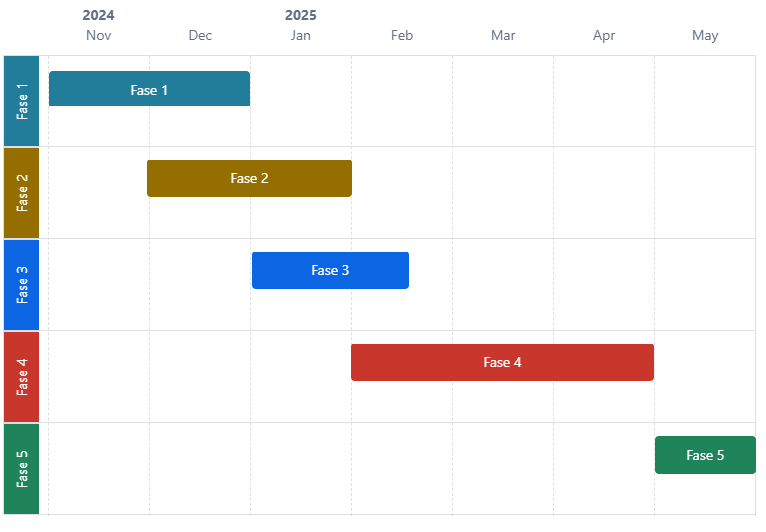
\includegraphics[width=.5\textwidth]{../graphics/Chart-Tijd-Visualisatie.png}
    \caption{Tijdsplanning van het project}
    \label{fig:tijdsplanning}
\end{figure}


%---------- Verwachte resultaten ----------------------------------------------
\section{Verwacht resultaat, conclusie}%
\label{sec:verwachte_resultaten}

De meerwaarde van deze bachelorproef voor de doelgroep, de Aquarius Zwemclub Lebbeke, is duidelijk: de implementatie van een robuuste cloudopslagoplossing zal niet alleen de werkprocessen voor de lesgevers verbeteren, maar ook de algehele efficiëntie van de club vergroten. Door de administratieve processen te automatiseren en beter beheersbaar te maken, wordt er tijdswinst geboekt, wat meer ruimte biedt voor de daadwerkelijke activiteiten van de club. Bovendien zal de verbetering van de toegang en beveiliging van documenten bijdragen aan een professionelere werking van de zwemclub.

De verwachte conclusie van deze bachelorproef is dan ook dat het gekozen cloudopslagsysteem zowel technisch haalbaar als praktisch effectief zal zijn voor de behoeften van de zwemclub. Mocht de gekozen oplossing echter niet voldoen aan de verwachtingen, dan zal het onderzoek zich richten op het identificeren van de tekortkomingen en de redenen waarom deze oplossing niet geschikt bleek. In dat geval zal er verder onderzocht worden welke alternatieven nog beter aansluiten bij de eisen van AZL.

%%---------- Andere bijlagen --------------------------------------------------
% TODO: Voeg hier eventuele andere bijlagen toe. Bv. als je deze BP voor de
% tweede keer indient, een overzicht van de verbeteringen t.o.v. het origineel.
%\input{...}

%%---------- Backmatter, referentielijst ---------------------------------------

\backmatter{}

\setlength\bibitemsep{2pt} %% Add Some space between the bibliograpy entries
\printbibliography[heading=bibintoc]

\end{document}
